\documentclass[a4paper,twocolumn,5p]{elsarticle}

\usepackage{hyperref}
%\usepackage{lineno}
%\modulolinenumbers[5]

\usepackage{booktabs}
\usepackage{graphicx}
\usepackage{xspace}
\usepackage{booktabs}
\usepackage[draft]{fixme}

\journal{Environment International}

%% `Elsevier LaTeX' style
\bibliographystyle{elsarticle-num}
%%%%%%%%%%%%%%%%%%%%%%%

\begin{document}

% Macro para escribir NO$_2$
\newcommand{\no}{NO\textsubscript{2}\xspace}

\begin{frontmatter}

\title{A comparison of probabilistic forecasting methods for extreme \no pollution episodes}

\author{Sebasti\'an P\'erez Vasseur} 
\address{Artificial Intelligence Department\\Universidad Nacional de
  Educaci\'on a Distancia --- UNED\\c/ Juan del Rosal, 16, Madrid, Spain}

\author{Jos\'e L. Aznarte\fnref{myfootnote}}
\address{Artificial Intelligence Department\\Universidad Nacional de
  Educaci\'on a Distancia --- UNED\\c/ Juan del Rosal, 16, Madrid, Spain}
\ead{jlaznarte@dia.uned.es}

\fntext[myfootnote]{This work has been partially funded by Ministerio
  de Econom\'ia y Competitividad, Gobierno de Espa\~na, through a
  \emph{Ram\'on y Cajal} grant % awarded to Dr Aznarte
  (reference: RYC-2012-11984).}


\begin{abstract}

\end{abstract}

\begin{keyword}
probabilistic forecasting \sep air quality \sep quantile regression
\sep nitrogen dioxide \sep Madrid
\end{keyword}

\end{frontmatter}

%\linenumbers

\section{Introduction}
\label{sec:intro}

Pollution has been become an increasing topic in cities due to their adverse 
effects on health and their increasing levels mainly due to human activity 
(traffic, heating systems, ...). Forecasting pollution levels is therefore needed 
in order to take preventive measures against it. More specifically, detecting pollution 
peaks beforehand could give cities enough time to take effective measures.

Multiple research papers have focused on this issue and have dealt with the
forecast of pullutants level. Bai et al. \cite{bai_air_2018} describes the latest 
state of the art in this exercise. As noted by them, there's a diverse range of 
solutions to this problem.

However as noted by Hothorn et al. \cite{hothorn_conditional_2014}, the real objective in a 
regression analysis is to find the conditional distribution of the target variable: in our 
case, the full distribution of the levels of the pollutants. Indeed, the full distribution 
gives an idea of the uncertainty of our predictions and can be useful to forecast the probability 
of the signal being above a certain health threshold. 
For example, $NO_2$ pollutant presence in the air is said to be harmful 
from 180 $\mu g / m^3$. 

Previous research \cite{proba_aznarte} has already focused on probabilistic forecasting
for the $NO_2$ pollutant levels.

This work focused on the horizon 1 (forecasting levels 1
hour before) and only used 1 type of model (Quantile Random Forest). We will 
extend this work by testing more models (Quantile linear regression, Gradient Boosted trees 
and K Neighbors) and for different horizons (up to 60 hours before). 
We will inspire our work on the techniques displayed during the GEFCom Competition 
\cite{mangalova_k-nearest_2016} \cite{hong_probabilistic_2016}.

Also we will improve the current models by applying a statistical inference to the output
of the models. This way, we are converting our forecasting method into a semi-parametric 
model.

\section{Probabilistic forecasting with quantile regression}
\label{sec:probForec}

The prediction from most regression models is a
point estimate of the conditional mean of a dependent variable, or
response, given a set of independent variables or predictors. However,
the conditional mean measures only the center of the conditional
distribution of the response, and if we need a more complete summary
of this distribution, for example in order to estimate the associated
uncertainty, quantiles are in order. The 0.5 quantile (i.e., the
median) can serve as a measure of the center, and the 0.9 quantile
marks the value of the response below which reside the 90\% of the
predicted points. Recent advances in computing have inducted the
development of regression models for predicting given quantiles of the
conditional distribution. The technique is called quantile regression
(QR) and was first proposed by Koenker in 1978
\cite{koenker_quantile_2001} based on the intuitions of the
astronomer and polymath Rudjer Boscovich in the 18th
century. Elaborating from the same concept of estimating conditional
quantiles from different perspectives, several statistical and CI
models that implement this technique have been developed: from the
original linear proposal to multiple or additive regression, neural
networks, support vector machines, random forests etc.

Quantile regression has gained an increasing attention from very
different scientific disciplines \cite{yu_quantile_2003}, including
financial and economic applications \cite{ben_rejeb_financial_2016},
medical applications \cite{jang_quantile_2018}, wind power
forecasting \cite{wan_direct_2017}, electric load forecasting
\cite{lebotsa_short_2018}, environmental modelling
\cite{cade_gentle_2003} and meteorological modelling
\cite{baur_modelling_2004} (these references are just
examples and the list is not exhaustive). To our knowledge, despite
its success in other areas, quantile regression has not been applied
in the framework of air quality , with the exception of
 \cite{martinezsilva_forecasting_2016}.

Thus, as we can estimate an arbitrary quantile and forecast its
values, we can also estimate the full conditional distribution, which
will entail us to the results presented in Section \ref{sec:results}.

Among the array of methods that allow to estimate and forecast
data-driven conditional quantiles, in this study we have chosen
linear quantile regression,
k-neighbors quantile regression, quantile regression forests and quantile XGBoost. 

We will compare the different algorithms through the CRPS metric for the 
distribution and the RMSE, MAE, Correlation and Bias for the quantile 50.

\section{Data description and experimental design}

\subsection{$NO_2$}
\label{sec:no2}
All of the 24 stations of Madrid’s monitoring system capture hourly data for NO2. 
They are spatially distributed according to European regulations.
We can see the station distribution in figure \ref{figure:stations}.

\begin{figure}
  \centering
      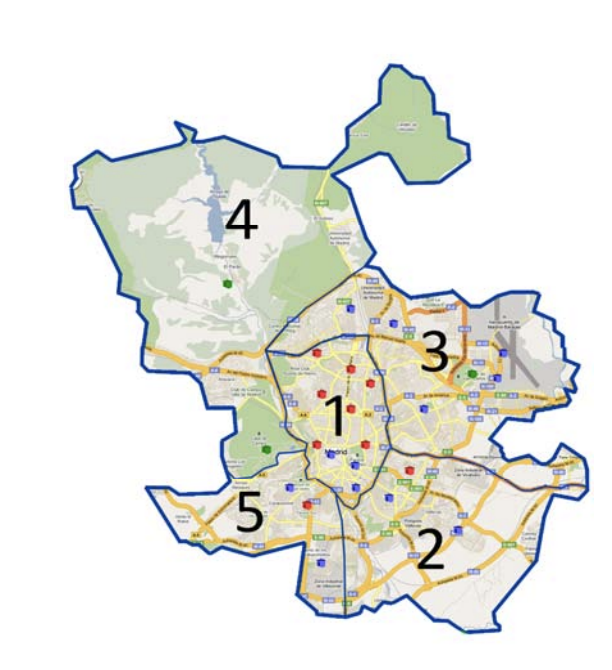
\includegraphics[width=0.4\textwidth]{zonas_madrid}
      \label{figure:stations}
  \caption{Madrid Pollution Stations and Zones.}
\end{figure} 

They are classified into 
three types: background stations, suburban stations 
and traffic stations. 

For this study, we have selected the Diaz Aguirre station.

After analysis of the $NO_2$ values (see \ref{figure:histo_no2}), the shape 
of the histogram approaches the one from a lognormal distribution 
and therefore we transformed to 
the log of the values. This has 2 positive effects: it reduces the tail of the 
distribution which will enable better quantile estimation and it reduces the 
skewness of the distribution 
which helps with linear models like the linear quantile regression.

\begin{figure}
  \centering
  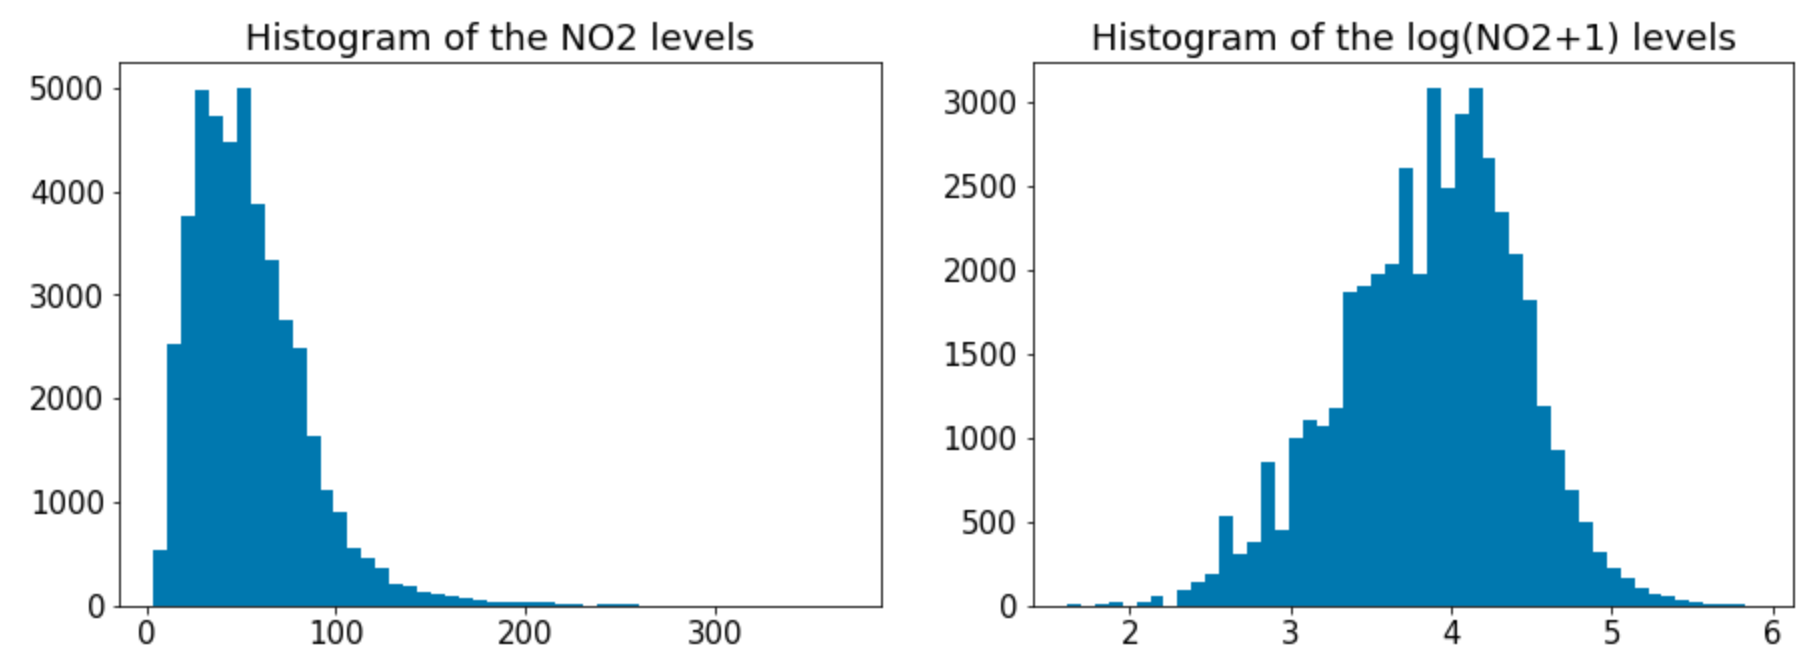
\includegraphics[width=0.4\textwidth]{histo_no2}
  \caption{Histogram of $NO_2$}
  \label{figure:histo_no2}
\end{figure}

The time series for this station consists of hourly
measured values of the airborne concentrations of NO2
from 01/01/2000 to 30/11/2017. These values exhibit a clear intraday 
pattern, in which the
higher values are located in two peaks around the morning
and evening (with highest average value at 19h) while the 
nightly hours (from 00h to 05h) have lower average concentrations. 
Not only are the values higher at those hours, but also
the variance is, as we can see in figure \ref{figure:variance}. 
 
\begin{figure}
  \centering
      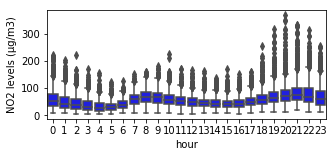
\includegraphics[width=0.4\textwidth]{NO2Var}
  \caption{Boxplot of NO2 per hour}
\label{figure:variance}
\end{figure}

In order to analyze the seasonality of the signal, we extract the 5 main factors 
from the Fourier Transform. Those can be seen clearly from the first 3000 components:

\begin{itemize}
  \item Every 12 hour Seasonality
  \item Yearly Seasonality
  \item Daily Seasonality
  \item Every 4 year seasonality
  \item Weekly Seasonality
\end{itemize} 

Therefore, we will create as input the output of periodic functions (cos and sin) whose frequency 
is equal to the ones found 
above. This will enable the machine learning model learn the seasonality of our time series.

As with any forecast technique based on machine learning, we add lagged values to improve the accuracy 
of the analysis. We are limited by the horizon of the prediction and 
keeping a reasonable number of features as input. We will take lagged values from the inmediate past (hours before)
and from past periods (based on the seasonal analysis): 1-5 hours before, values on the 9 days before at the same 
hour and values on the 9 days and 12 hours before.

\subsection{$O_3$}

The Diaz Aguirre station also recorded the levels of $O_3$. As we can see in figure \ref{figure:no2vso3},
there seems to be a correlation between $NO_2$ levels and $O_3$.

\begin{figure}
  \centering
  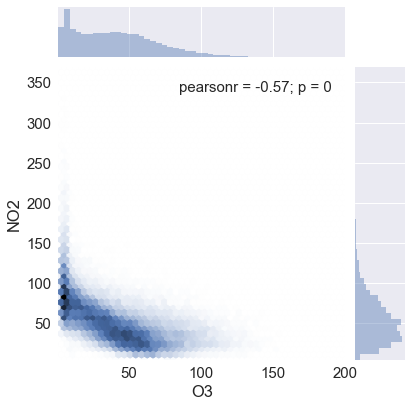
\includegraphics[width=0.4\textwidth]{no2vso3}
  \label{figure:no2vso3}
  \caption{Levels of $O_3$ vs levels os $NO_2$}
\end{figure}

We will also add lagged values of $O_3$ to our models.

\subsection{ECMWF numerical pollution prediction}
\label{sec:ecmwf-numer-poll}

The European Centre for Medium-Range Weather Forecasts implements the Copernicus Atmosphere Monitoring Service.
This service provides CAMS delivers a saily production of near-real-time European air quality analyses and forecasts 
with a multi-model ensemble system. 
As you can see in the figure \ref{figure:camspoints}, the scope of the forecast is european and does not have the needed granularity to forecast 
the levels of NO2 in a station.

\begin{figure}
  \centering
  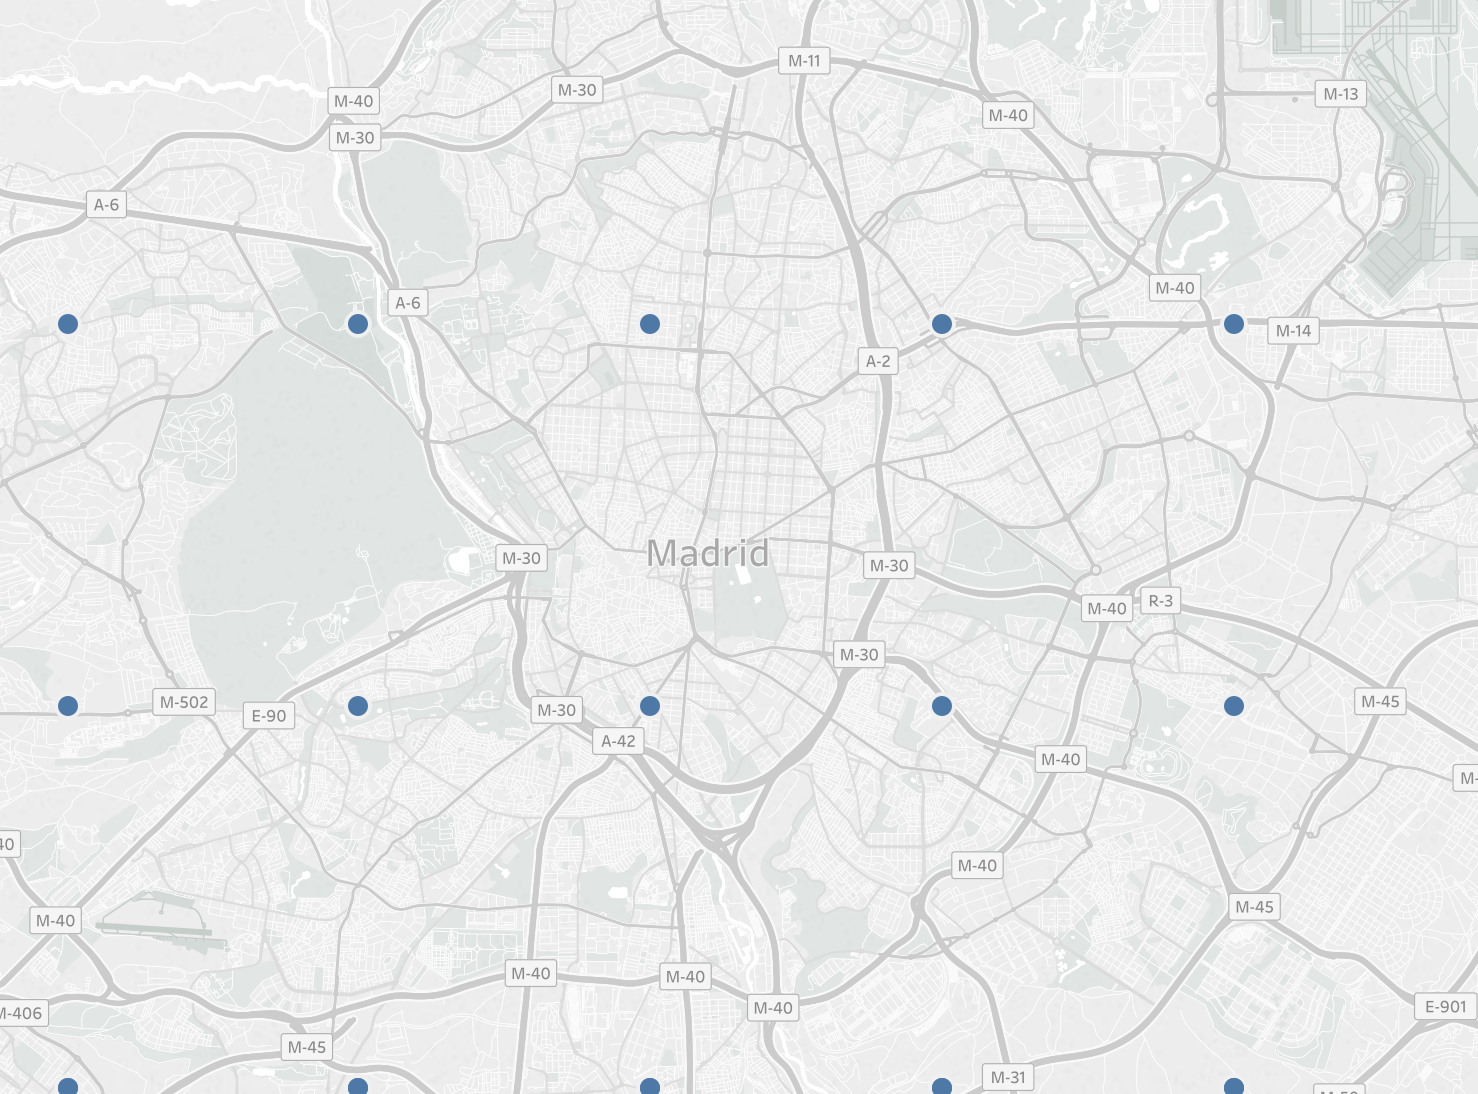
\includegraphics[width=0.4\textwidth]{camspoints}
  \label{figure:camspoints}
  \caption{Location of the points with predicted pollution from CAMS.}
\end{figure}

\subsection{Calendar Variables}
\label{sec:cal_data}

As $NO_2$ levels seem to be linked to human activity, we will also flag the hours 
belonging to a specific type of day. Days could be classified as:
\begin{itemize}
  \item Bank holidays
  \item Heavy traffic day (for example, return from holidays)
  \item School holidays
\end{itemize} 

We will also input past values of this variables (up to 3 days before).

\subsection{Experimental Design}
\label{sec:experimental-design}

First, we aligned and gathered all the hourly time series: $NO_2$, $O_3$, ECMWF and calendar variables.
Then we transformed the signal levels and then we added the lagged values 
and a seasonal time series with the 
main periods of the $NO_2$ time series. 
Table summarizes the predictors we will use in this exercise.

Once all this data is added, we will train the following probabilistic 
models:
\begin{itemize}
  \item Quantile Random Forest (RF)
  \item $k$ Nearest Neighbors (KNN)
  \item Linear Quantile regression (QLR)
  \item Quantile Gradient Boosting (GB)
\end{itemize}

The figure \ref{figure:dataflow} shows the data flow in the experimental design.  

\begin{figure}
  \centering
  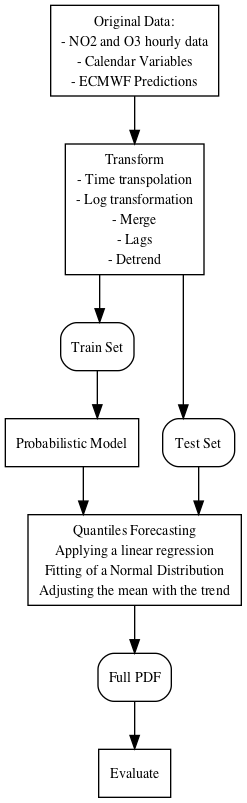
\includegraphics[width=0.2\textwidth]{diagrams/flow}
  \caption{Data flow of the experiments}
  \label{figure:dataflow}
\end{figure}

The section \ref{sec:models} provides more information on the probabilistic models.

As explained by Bergmeir et al \cite{bergmeir_note_2018}, there are several methods
to separate the train and test set. We will use the Out-of-sample method:
We will train the models with data prior to 2017 and we will test our 
models with 2017 data. We will always test with 
predictions done at 10:00, as this is the time the 
forecast will be done as the data is available at that time.

After forecasting the quantiles, we will fit those quantiles to a normal distribution.

Fitting a normal distribution to those percentiles and then generating the 
percentiles for that fitted distribution has several advantages. It lets to build a 
fine grained distribution if you do not have enough percentiles.
It helps estimating the upper tail of the distribution, in spite of the 
low probability for 
those values.

We will evaluate the 50 percentile through standard evaluation metrics like: RMSE, MAE, 
Bias and Corr 
and the whole forecasted CDF through the CRPS. We will perform
this evaluation for each of the models and each of the horizons.

\subsection{Probabilistic Models}
\label{sec:models}

We will compare the following probabilistic models:
\begin{itemize}
  \item Quantile Random Forest
  \item $k$ Nearest Neighbors
  \item Linear Quantile regression
  \item Quantile Gradient Boosting 
\end{itemize}

\subsubsection{Quantile Random Forest}

Quantile random forests create probabilistic predictions out of 
the original observations. It works like the usual random forest, 
except in each tree,
leafs do not contain a single value as a prediction but the target observations 
from the training set 
belonging to that leaf (see figure \ref{figure:qrandom}) . 

Then predictions are calculated by selecting the leafs in each tree
corresponding to the input features and combining the weighted 
histograms in each tree out of the target observations in those leafs. 
For more information refer to 
\cite{quantregforests}.

However, Quantile Random Forest does not provide good results. We believe this is 
due to the high linear dependence between the input predictors and the target. 
We observe this linearity while comparing the performance of a linear regression and 
a random forest for a standard forecast, as we can see 

We decided to train a linear regressor
which predicts the $NO_2$ values mean and use the Quantile 
Random Forest to predict the full distribution of the residuals of that linear regression.
Diagram  shows the updated process.  

\begin{figure}
  \centering
  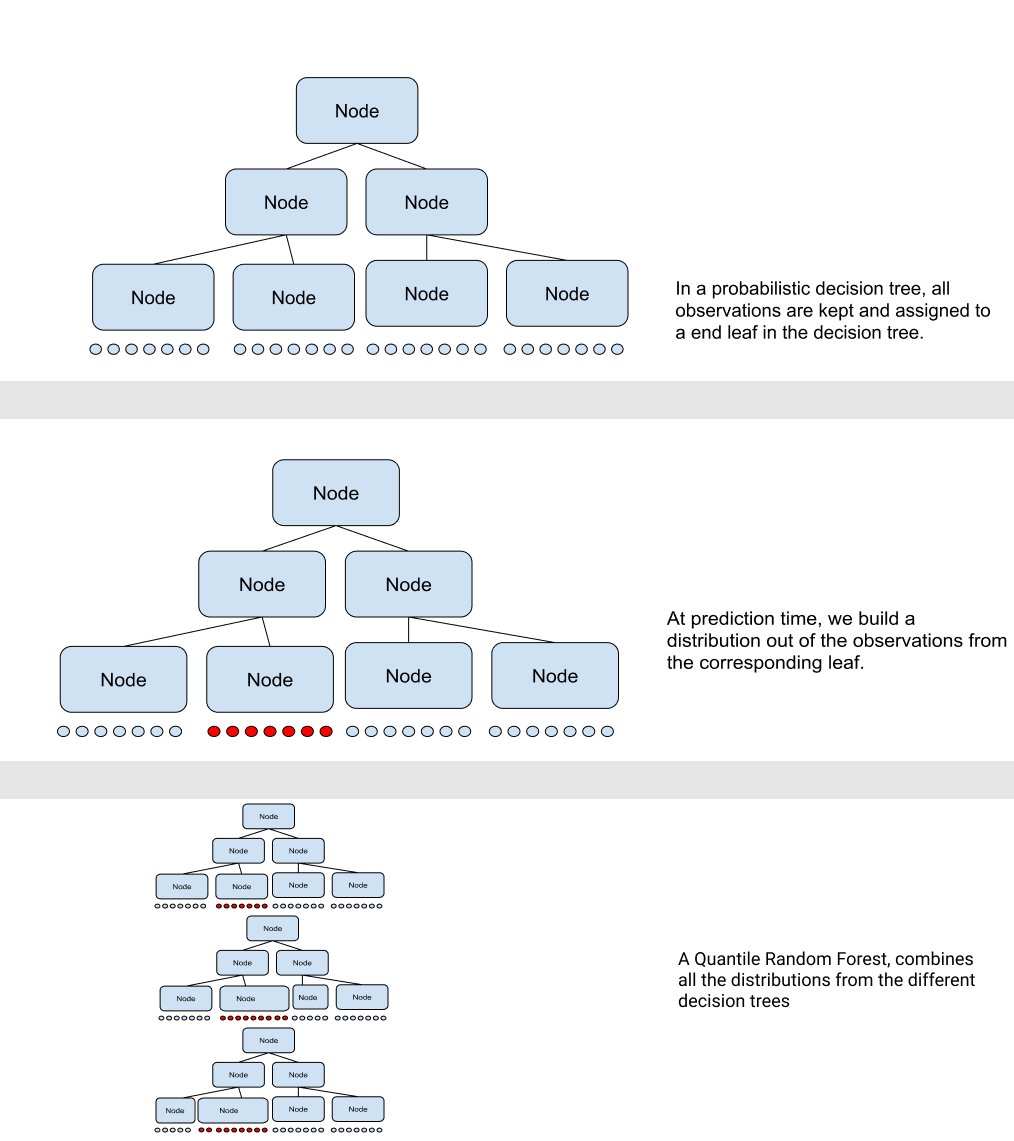
\includegraphics[width=0.4\textwidth]{quantile_random_forest}
  \caption{Random Forest Weights on observations based on trained trees}
  \label{figure:qrandom}
\end{figure}

\subsubsection{$k$ Nearest Neighbors}

We will use the probabilistic $k$ nearest neighbors algorithm as described in  
\cite{quantileknnmangalova}. 
This algorithm is based on the standard $k$ nearest neighbor, 
where instead of calculating the mean of 
the targets of the
$k$ nearest points to the input, it builds a distribution 
from those neighbors.

We found the best $k$ to be 50 after testing several values of $k$.

In order to obtain better results, we also applied the same process as for 
quantile random forest by predicting the full distribution of the residuals 
of a linear regression.

\subsubsection{Linear Quantile regression}

We can apply linear regression with a modified cost function in order to 
predict the quantiles of the target (for a detailed discussion of 
quantile regression, refer to \cite{koenker_quantile_2001}). 

Given a 
set of vectors $(x_i, y_i)$, in point forecasting we are usually 
interested in what prediction $\hat y(x) = \alpha_0 + \alpha_1 x$
minimizes the mean squared error,
\begin{equation}
  \label{eq:1}
  E = \frac{1}{n} \sum^n_i \epsilon_i =
  \frac{1}{n} \sum^n_i [ y_i - (\alpha_0 + \alpha_1 x) ]^2.
\end{equation}
This prediction is the conditional sample mean of $y$ given $x$ , that
 is, $\hat y(x) = \hat\alpha_0 + \hat\alpha_1 x$
, or the location of the conditional distribution. But we could be
interested in estimating the conditional median (i.e., the 0.5
quantile) instead of the mean, in which case we should find the
prediction $\hat y(x)$ which minimizes the mean absolute error,
\begin{equation}
  \label{eq:2}
  E = \frac{1}{n} \sum^n_i \epsilon_i =
  \frac{1}{n} \sum^n_i | y_i - (\alpha_0 + \alpha_1 x) |.
\end{equation}
The fact is that, apart from the 0.5 quantile, it is possible to
estimate any other given quantile $\tau$. In that case, instead of
(\ref{eq:2}), we could minimize
\begin{equation}
  \label{eq:3}
E= \frac{1}{n} \sum^n_i f( y_i - (\alpha_0 + \alpha_1 x))
\end{equation}
where
\begin{equation}
  \label{eq:4}
  f(y-q) = \left\{ 
\begin{array}{l l}
\tau (y-q) & \quad \mbox{if $y \ge q$}\\
(1-\tau) (q-y) & \quad \mbox{if $y < q$}\\
\end{array} \right.,
\end{equation}
with $\tau \in (0,1)$. Equation (\ref{eq:3}) represents the
median when $\tau=0.5$ and the $\tau$-th quantile in any other case.

We will train 5 models to predict the 5 deciles of the signal. As quantiles are 
calculated separately, we have the risk of encountering quantile crossing.
We will use the simple technique as explained in \cite{cross} to solve this problem.

\subsubsection{Gradient Boosted Tree}

Tree Boosting \cite{friedman_greedy_2001} is a widely used technique for machine learning 
that consist on growing trees based on the compromise 
of a cost function and a regularization function. This cost function is usually 
used to forecast 
the mean of the signal. We will modify the cost function (im a similar way as in 
the quantile linear regression) to predict the quantiles of the target. 

We will train 5 models to predict the 5 deciles of the signal and we will solve 
 quantile crossing with the technique explained in \cite{cross}. 

\section{Results and discussion}
\label{sec:results}

\begin{figure*}
  \centering
  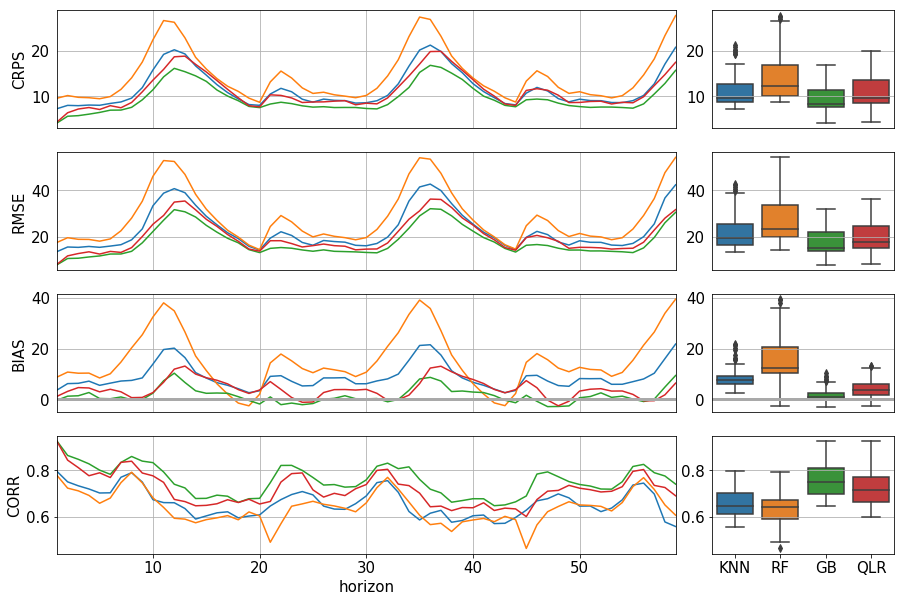
\includegraphics[width=\textwidth]{results/errorGraph}
  \caption{Continuous ranked probability score, root mean squared
    error and bias of the different models with respect to the
    forecasting horizon and in average.}
  \label{figure:errorGraph}
\end{figure*}

Figure \ref{figure:rel_sharp} shows the average reliability and sharpness of the 
different methods across all the horizons. 
As we can see, Random Forest and Kneighbors display a high bias that can be seen in the 
sharpness curve. QLR results give a hint on why this is happening. It seems the relationship
between the target and the input variable is highly linear, therefore models like Random 
Forest and Kneighbors suffer from that. Gradient Boosting performs the best of all.

\begin{figure*}
  \centering
  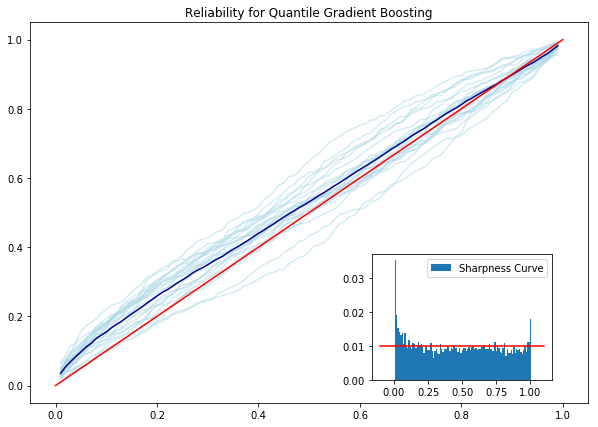
\includegraphics[width=1\textwidth]{reliability_sharpness}
  \caption{Average Reliability and Sharpness of the different probabilistic forecasting
  across all horizons}
  \label{figure:rel_sharp}
\end{figure*}

\begin{table}[tbp]
  \centering
  \label{tab:determ}
  \caption{CRPS Error for the different methods at different
    horizons (GB = Gradient Boosting,
    KNN = K Nearest Neighbor,
    LQR = Linear Quantile Regression,
    QRF = Quantile Random Forest)
    }
    \begin{tabular}{lrrrrrrr}
      \toprule
      method &  Arima &    GB &   GBL &   KNN &   QLR &    RF &   RFL \\
      horizon &        &       &       &       &       &       &       \\
      \midrule
      1       &   6.18 &  4.00 &  3.97 &  4.65 &  4.16 &  7.73 &  4.21 \\
      12      &  13.52 & 15.35 & 15.87 & 16.99 & 18.17 & 21.59 & 16.48 \\
      13      &  12.83 & 15.25 & 15.85 & 16.96 & 18.62 & 19.70 & 16.55 \\
      14      &  11.54 & 14.38 & 14.19 & 15.41 & 16.75 & 16.53 & 14.92 \\
      20      &   7.11 &  7.31 &  7.16 &  7.51 &  7.51 &  8.05 &  7.18 \\
      37      &  13.31 & 15.82 & 16.48 & 17.92 & 19.19 & 20.13 & 16.94 \\
      45      &   9.01 &  9.27 &  9.71 & 11.14 & 11.29 & 12.40 & 10.28 \\
      55      &   6.22 &  7.23 &  7.71 & 10.58 &  8.20 & 10.20 &  8.27 \\
      \bottomrule
      \end{tabular}
      
  
\end{table}


Table \ref{tab:determ} shows GB outperforms the other Machine Learning algorithms.


\section{Conclusions}
\label{sec:concl}

\section{References}

\bibliography{refs}

\end{document} 
%%% Local Variables:
%%% mode: latex
%%% TeX-master: t
%%% End:
